\documentclass[a4paper]{article}
\usepackage{times}
\usepackage[utf8]{inputenc}
\usepackage[T1]{fontenc}
\usepackage{graphicx}
\usepackage{amssymb}
\usepackage{hyperref}
\linespread{1.5}	% double spaces lines
\usepackage[hmargin=3cm,vmargin=3cm]{geometry}
\usepackage{indentfirst}
\usepackage{amsmath}
\usepackage{amsthm}
\usepackage{sectsty}
\usepackage{enumitem}
\usepackage[brazil]{babel}
\usepackage{placeins} %mantem figuras na secao com \FloatBarrier
\usepackage{fixltx2e} %\textsubscript
\usepackage{textcomp}
\hypersetup{%
    pdfborder = {0 0 0}
}

\begin{document}

\begin{titlepage}
\begin{center}


\large{ 
\uppercase{ Universidade Federal do Rio Grande do Sul\\

Instituto de Informática \\

Curso de Ciência da Computação \\

Teoria da Computação N (2014/1)\\
}

Prof. Dr. Tiarajú Asmuz Diverio \\


Graduandos: \\ Paulo Renato Lanzarin, Ricardo Gabriel Herdt (Turma C) e \\
	Wladimir Leuschner (Turma B) \\[4.5cm]



% Title
\LARGE {\bfseries Autômato com Duas Pilhas para \\
	reconhecer a linguagem ww \\[1.0cm]
}}


\vfill

Porto Alegre, 05 de abril de 2014

\end{center}
\end{titlepage}

A máquina para reconhecer a linguagem \textbf{ww} é definida por

$M = (\{a, b\}, \{q0, q1, q2, .., q15, qf\}, \Pi, q0, \{qf\}, \{A, B, C, D, E\})$, 

onde $\Pi$ é a função programa representada através do seguinte grafo:

\begin{figure}[h!]
  \centering
  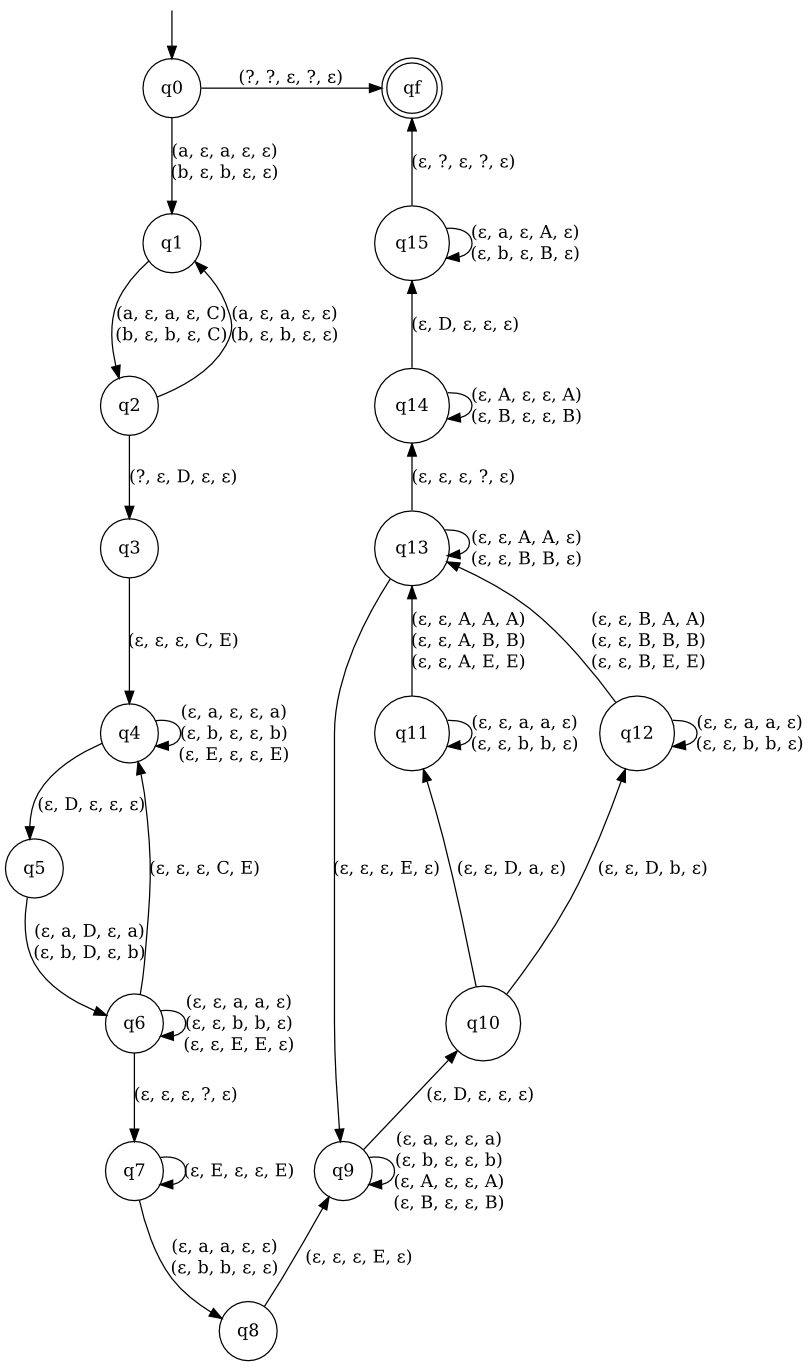
\includegraphics[scale=0.55]{ww_pilhas.png}
\end{figure}

\end{document}
